\documentclass[noamsthm,8pt,t,xcolor={dvipsnames}]{beamer}

\mode<presentation>{\usetheme{CEITEC}}

\usepackage[english]{babel}
\usepackage[mathletters]{ucs}
\usepackage[utf8x]{inputenc}
%\usepackage{unimath}
\usepackage{helvet}
\RequirePackage{amssymb}
\usepackage{amsmath}
\usepackage[T1]{fontenc}
\usepackage{fleqn}
\usepackage{graphics}
\usepackage{fixltx2e}
\usepackage{multicol}
\usepackage{cancel}
\usepackage{eurosym}

\definecolor{mygreen}{rgb}{0.92,1,0.82}

\setbeamertemplate{blocks}[rounded][shadow=true]
\setbeamercolor*{block title}{fg=white, bg=ceitecprimary}
\setbeamercolor*{block body}{fg=black, bg=mygreen}

\makeatletter
\def\@ptsize{100}
\def\ie{i.\,e.\ \ignorespaces}
\def\eg{e.\,g.\ \ignorespaces}
\def\TiSiO{Ti\textsubscript{x}Si\textsubscript{1--\itshape x}O\textsubscript{2}}
\def\TiO2{Ti\textsubscript{2}}
\def\SiO2{Si\textsubscript{2}}
\parindent=0pt

\def\graphframe#1#2{%
  \begin{frame}
  \frametitle{#1}
  \includegraphics[width=\hsize]{#2.pdf}
  \end{frame}
}

\setbeamersize{text margin left=2.5em}
\setbeamersize{text margin right=2.5em}

\renewcommand\footnoterule{\rule{\linewidth}{0pt}}

\title[Optical properties of \TiSiO{}]
      {{\textit Ab initio} calculations of optical response and core-level XPS spectra in \TiSiO}
\author[Pavel Ondračka]
       {\underline{Pavel Ondračka}\inst{1,2} \and David Holec\inst{3} \and David Nečas\inst{1} \and Eva Kedroňová\inst{1,2} \and Stéphane Elisabeth\inst{4} \and Mireille Richard\inst{4} \and Antoine Goullet\inst{4} \and Lenka Zajíčková\inst{1,2}}
\institute[Masaryk University]
          {{\inst{1} RG Plasma Technologies, Central European Institute of Technology, Masaryk University, Brno, Czech Republic\\
         \inst{2} Department of Physical Electronics, Faculty of Science, Masaryk University, Brno, Czech Republic \\
         \inst{3} Department of Physical Metallurgy and Materials Testing, Montanuniversität Leoben, Leoben, Austria\\
         \inst{4} Institut des Matériaux Jean Rouxel (IMN), Université de Nantes, Nantes, France
}}

\date[] % (optional)
{Brno, 8 December 2016}

\begin{document}

\frame[plain]{%
\titlepage
}

\section*{Outline}

\begin{frame}
\frametitle{Outline}
  \tableofcontents
\vskip 0pt plus4fill
\end{frame}

\section{\TiSiO{} showcase}

\begin{frame}
   \frametitle{\TiSiO{} showcase}
   \begin{columns}
      \begin{column}{0.6\textwidth}
         \vspace{1cm}
         \begin{itemize}
            \item Big difference between optical and electronic properties
            \item Refractive index: TiO$_2$ $>$2.5, SiO$_2$ $\sim$1.5
            \item Band gap: TiO$_2$ 3.0--3.5\,eV, SiO$_2$ $\sim$9\,eV
            \item Static dielectric function TiO$_2$ $\sim$80, SiO$_2$ $\sim$3.9
            \item Fine-tuning properties by composition change brings new possibilities in design of optical devices (filters, anti-reflective coatings, ...)
         \end{itemize}
      \end{column}
      \begin{column}{0.4\textwidth}
         \begin{center}
            TiO$_2$
            \includegraphics[width=\linewidth]{figures/SEM-Xsection-TiO2.png}
            \vspace{0.3cm}
            SiO$_2$
            \includegraphics[width=\linewidth]{figures/SEM-Xsection-SiO2.png}
         \end{center}
      \end{column}
   \end{columns}
\end{frame}

\subsection{Modelling introduction}
\begin{frame}
   \frametitle{Construction of structural models}
   \vspace{-0.3cm}
   \begin{columns}
      \begin{column}{0.8\textwidth}
         \begin{itemize}
            \item Density Functional Theory
            \item Vienna Ab initio Simulation Package (pseudopotential plane wave DFT code)
            \item Standard GGA PBE exchange-correlation functional
            \item Structure sizes around 100 atoms
         \end{itemize}
      \end{column}
      \begin{column}{0.2\textwidth}
         \begin{center}
            \includegraphics[width=0.9\linewidth]{figures/VASP.jpg}
         \end{center}
      \end{column}
   \end{columns}

   \pause

   \begin{columns}
      \begin{column}{0.5\textwidth}
         \begin{center}
             \includegraphics[width=0.6\linewidth]{figures/SQS.png}
         \end{center}
         \begin{itemize}
            \item Crystalline solid solutions with Special Quasirandom Structures (SQS) methods
            \item Based on anatase, rutile and selected SiO$_2$ structures
         \end{itemize}
      \end{column}

      \pause

      \begin{column}{0.5\textwidth}
         \begin{center}
            \includegraphics[width=0.5\linewidth]{figures/am-SA.png}
         \end{center}
         \begin{itemize}
            \item Amorphous structures prepared by ab-initio simulated annealing (SA)
            \item Annealed at 3000\,K for 3\,ps than cooled to 0K over 3\,ps and relaxed
         \end{itemize}
      \end{column}
   \end{columns}
\end{frame}

\begin{frame}
   \frametitle{Structural stability}
   \begin{columns}
      \begin{column}{0.55\textwidth}
         \vspace{-0.85cm}
         \begin{center}
            \includegraphics[width=\linewidth]{figures/Ef-all.pdf}
         \end{center}
      \end{column}
      \begin{column}{0.45\textwidth}
         \begin{center}
            \only<1-2>{
               \includegraphics[width=\linewidth]{figures/coord.pdf}
            }
            \only<3>{
               \includegraphics[height=4cm]{figures/phase.png}
            }
         \end{center}
      \end{column}
   \end{columns}

   \begin{itemize}
      \item SiO$_2$ like structures are more preferable (4-coordinated tetrahedral position)
      \item Amorphous structures less stable (at 0K)
      \item<2-> Known problem with TiO$_2$ stable structure prediction for both LDA and GGA 
      \item<2-> LDA+U/GGA+U helps\footnotemark, as well as some hybrids
      \item<3> Preference for separate phases, in agreement with phase diagram\footnotemark
   \end{itemize}
   \footnotetext[1]{Vu, N. H. et al., J. Phys. Condens. Matter 24, 405501 (2012).}
   \only<3>{
      \footnotetext[2]{\url{http://materials.springer.com/isp/phase-diagram/docs/c_0201188}}
   }
\end{frame}

\subsection{Band gap problems}
\begin{frame}
   \frametitle{Band gap problem}
   \framesubtitle{How to get a band gap cosistent with experiment}

   \vspace{-0.2cm}
   Notorious DFT (LDA/GGA) problem in band gap underestimation
   \begin{itemize}
      \item Possible ways to fix include scissor operator, DFT+U, hybrid and many body perturbation theory based approaches
      \item Hybrids and GW not feasible for large cells
   \end{itemize}

   \pause

   \emph{TB-mBJ exchange potential}$^1$ in combination with LDA-correlation offers solution
   \begin{itemize}
      \item<2-> Contains empirical parameters tuned for band gap value on large set of solids 
      \item<3-> Was already tested for optical properties of pure TiO$_2$ and found in reasonable agreement$^2$
      \item<3-> Improved TB-mBJ parametrisations$^3$ offer even better experimental agreement
      \item<3-> TB-mBJ and optical calculations done in Wien2k (all electron full-potential DFT code)
   \end{itemize}

   \only<2>{
      \vspace{-1.8cm}
      \begin{center}
         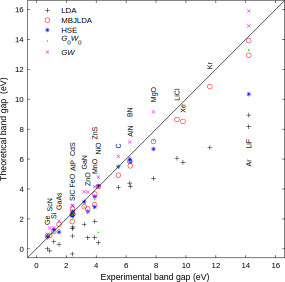
\includegraphics[width=4.65cm]{figures/mBJ.pdf}
      \end{center}
   }
   
   \only<2->{
      \footnotetext[1]{Tran, F. \& Blaha, P., Phys. Rev. Lett. 102, 226401 (2009).}
   }
   \only<3->{
      \footnotetext[2]{Gong, S. \& Liu, B.-G., Chinese Phys. B 21, 057104 (2012).}
      \footnotetext[3]{Koller, D., Tran, F. \& Blaha, P., Phys. Rev. B 85, 155109 (2012).}
   }
\end{frame}

\begin{frame}
   \frametitle{Band gap evolution}
   \framesubtitle{What happens when we add silicon into titania}

   \begin{columns}
      \begin{column}{0.5\textwidth}
         \begin{center}
            \includegraphics[width=\linewidth]{figures/gap1.pdf}
            \only<2->{
               \includegraphics[width=\linewidth]{figures/SiTiO2-dos.pdf}
            }
         \end{center}
      \end{column}
      \begin{column}{0.5\textwidth}
         \begin{itemize}
            \item Band gap (HOMO-LUMO like) actually decreases when Si is added
            \item This is observable for all structures
            \item<2-> States appear below and above the valence band
            \item<3> Si-induced oxygen states
         \end{itemize}
         \begin{center}
            \only<3>{
               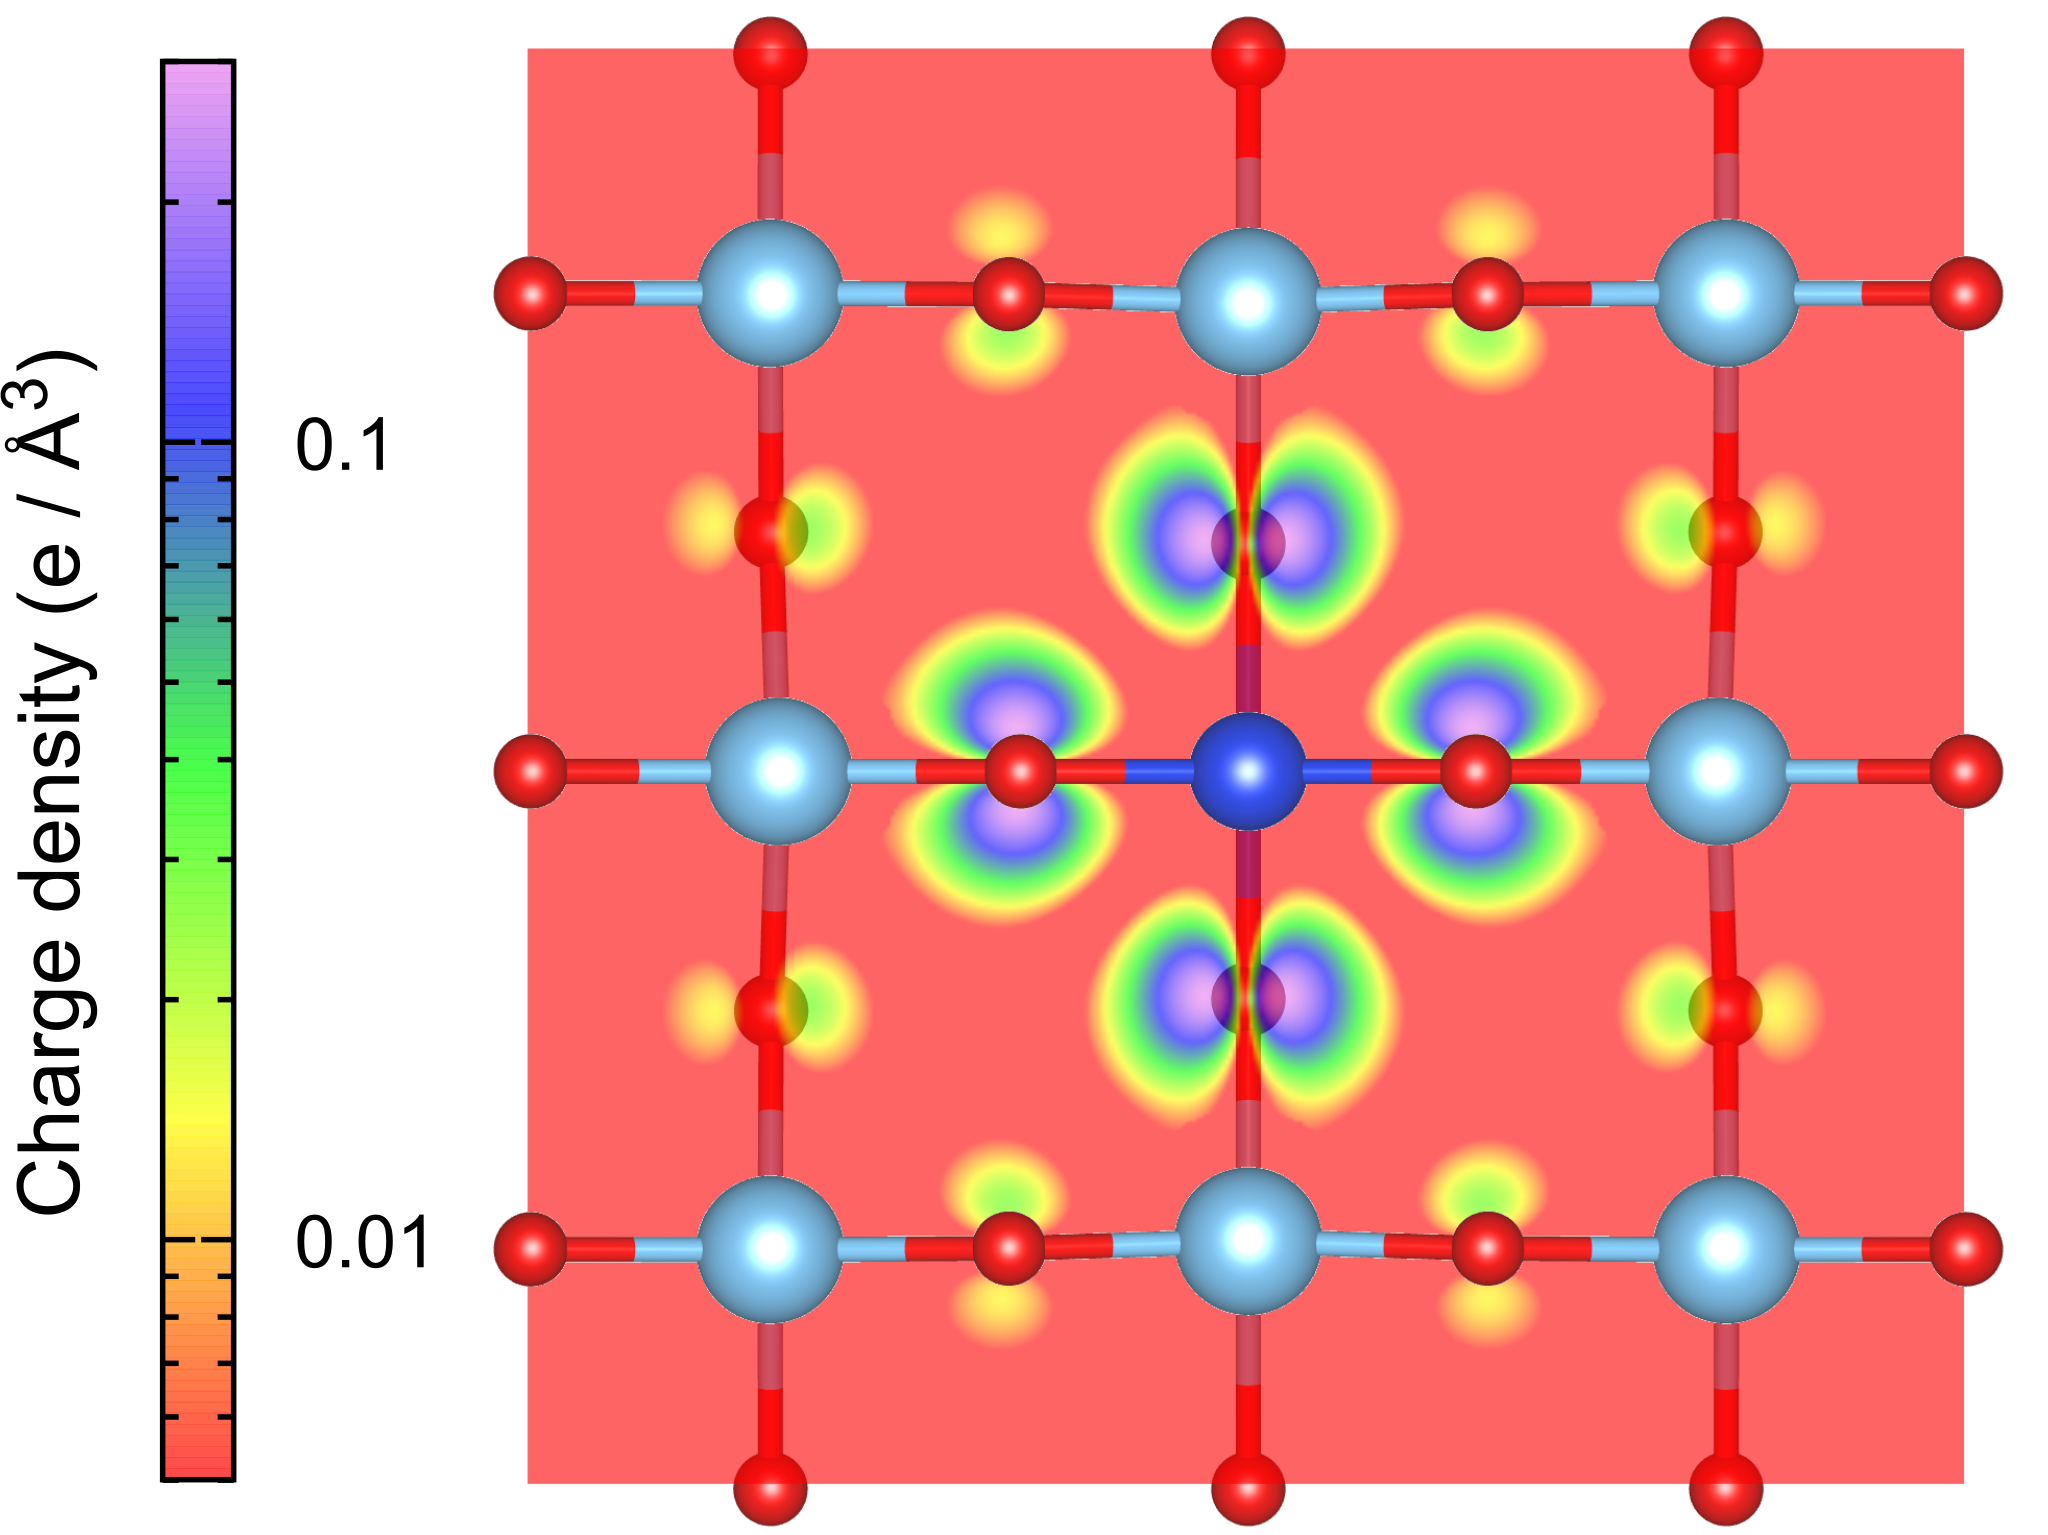
\includegraphics[width=\linewidth]{figures/charge-final.pdf}
            }
         \end{center}
      \end{column}
   \end{columns}
\end{frame}

\begin{frame}
   \frametitle{Band gap evolution}
   \framesubtitle{How to filter out the localized defect states}

   \begin{columns}
      \begin{column}{0.5\textwidth}
         Localized states observed also in the amorphous structures near the edge of valence and conduction band
         \begin{center}
            \includegraphics[width=\linewidth]{figures/IPR.pdf}
         \end{center}
      \end{column}
      \pause
      \begin{column}{0.5\textwidth}
         Band gap without localized states was estimated by an approach similar to Tauc plot
         \begin{center}
            \includegraphics[width=\linewidth]{figures/gap-edge.pdf}
         \end{center}
      \end{column}
   \end{columns}
\end{frame}

\subsection{Experimental setup}

\begin{frame}
   \frametitle{Deposition and characterisation}

   \begin{columns}
      \begin{column}{0.5\textwidth}
         Deposition
         \begin{itemize}
         \item \TiSiO{} thin films deposited by PECVD on c-Si
         \item Precursor gasses Titanium isopropoxide and Hexamethyldisiloxane
         \item<2-> ICP PECVD reactor, $p = 3$\,mTorr, $P = 400$\,W
      \end{itemize}
      \only<1>{
         \begin{center}
            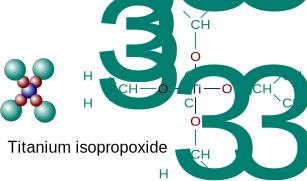
\includegraphics[width=0.6\linewidth]{figures/TTIP.pdf}
            \vspace{0.4cm}
            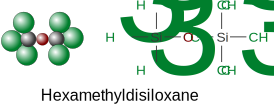
\includegraphics[width=0.6\linewidth]{figures/HMDSO.pdf}
         \end{center}
      }
      \only<2->{
         \begin{center}
            \includegraphics[width=1.0\linewidth]{figures/PECVD-reactor.pdf}
         \end{center}
      }
      \end{column}
      \begin{column}{0.5\textwidth}
         \only<3>{
            Optical characterisation
            \begin{itemize}
               \item Characterization done in spectral region up to 8.7eV
               \item Variable angle ellipsometry
               \item So-called Universal dispersion model was used$^1$
               \item Roughness (Rayleigh-Rice theory) and inhomogeneity included in the structural model
               \item NewAD fitting software
            \end{itemize}
            Composition and stochiometry determined by XPS, crystallinity by XRD
         }
         \end{column}
   \end{columns}
   \only<3>{
      \footnotetext[1]{Franta, D., Nečas, D. \& Ohlídal, I., Appl. Opt. 54, 9108 (2015).}
   }
\end{frame}

\subsection{Optical properties}

\begin{frame}
   \frametitle{Dielectric function}

   \begin{columns}
      \begin{column}{0.3\textwidth}
         \begin{itemize}
            \item Dielectric function calculated with Wien2k optic module 
            \item Calculation at the Random Phase Approximation level, e.g. no excitonic effects
            \item Good match of intensity, slight shift of peaks maxima
         \end{itemize}
      \end{column}
      \begin{column}{0.7\textwidth}
         \begin{center}
            \includegraphics[width=\linewidth]{figures/epsi-all.pdf}
         \end{center}
      \end{column}
   \end{columns}
\end{frame}

\begin{frame}
   \frametitle{Band gap}
   \framesubtitle{Comparison with experiment}

   \begin{center}
      \only<1>{
         \includegraphics[width=0.6\linewidth]{figures/gap2.pdf}
      }
      \only<2>{
         \includegraphics[width=0.6\linewidth]{figures/gap3.pdf}
      }
   \end{center}

   \begin{itemize}
      \item Experimental optical band gap increases slowly from value 3.26\,eV for pure TiO$_2$ and only after $x = 0.5$ goes up more sharply to $\sim$8.0\,eV for pure SiO$_2$
      \item<2> Almost perfect agreement for the calculated band gap of a-\TiSiO{} with experimental optical band gap after filtering out the localized states near band edges
   \end{itemize}
\end{frame}

\begin{frame}
\frametitle{Refractive index}
   \begin{columns}
      \begin{column}{0.7\textwidth}
         \vspace{-0.8cm}
         \begin{center}
            \includegraphics[width=0.8\linewidth]{figures/SiTiO2-n.pdf}

            \only<2>{
               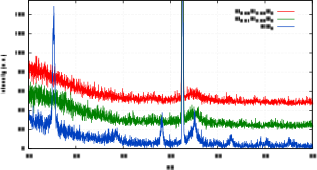
\includegraphics[width=0.7\linewidth]{figures/XRD.png}
            }
         \end{center}
      \end{column}
      \begin{column}{0.3\textwidth}
            \begin{itemize}
               \item Refractive index decreases approximately linearly in whole composition range
               \item Perfect agreement with experimental refractive index for a-\TiSiO{} again
               \item<2> By comparison with XRD we confirm the film are indeed amorphous except for pure TiO$_2$ where we have an anatase phase.
            \end{itemize}
      \end{column}
   \end{columns}
\end{frame}

\subsection{Phase separation problem}

\begin{frame}
   \frametitle{Phase separation problem}
   \vspace{-0.3cm}
   \begin{itemize}
      \item Phase separation into TiO$_2$/SiO$_2$ domains observed with samples deposited under energetic bombardment
      \item We hope to quantify this by fitting the O 1s peak into Ti--O--Ti, Ti--O--Si and Si--O--Si parts and also the Ti/Si 2p peaks into TiO$_2$/SiO$_2$ and Ti--O--Si mixed peaks
      \item Fixed peak shapes for TiO$_2$ and SiO$_2$ subpeaks obtained from pure materials
      \item Fitting is ambiguous without some constraints due to the broad nature of the individual peaks
      \item Fixed shifts and ratios between the TiO$_2$/SiO$_2$ parts of the O1s and Ti2p/Si2p peaks
   \end{itemize}
   \begin{center}
      \includegraphics[width=0.35\linewidth]{figures/XPSexp.pdf}
      \hspace{0.2cm}\vspace{-1cm}   
      \includegraphics[width=0.37\linewidth]{figures/XPSfit.pdf}
   \end{center}

\end{frame}

\begin{frame}
   \frametitle{Phase separation results}
   \vspace{-0.3cm}
   \begin{center}
      \includegraphics[width=0.8\linewidth]{figures/O1s-fit-delta.pdf}
   \end{center}
   \begin{itemize}
      \item The preliminary results seems promissing, more work is needed to generalize the formula for 3D
      \item !!!! Are the constraints reasonable? !!!!
   \end{itemize}
\end{frame}

\subsection{XPS spectra modelling}

\begin{frame}
   \frametitle{XPS spectra modelling}
   \vspace{-0.3cm}
   \begin{itemize}
      \item Slater's transition state approach: $$E_\mathrm{b} \approx -\frac{ \partial E_\mathrm{tot}(N − 0.5)} { \partial n_i} = −\epsilon_i(N − 0.5)$$
      \item Use this to calculate $E_\mathrm{b}$ for O 1s and Ti/Si 2p core states in the amorphous structure (with PBE).
      \item Replace the discrete energies with gausians to get spectra
   \end{itemize}
   \begin{center}
      \includegraphics[width=0.8\linewidth]{figures/XPS.pdf}
   \end{center}
\end{frame}

\begin{frame}
   \frametitle{Analysis of the calculated spectra}
   \vspace{-0.3cm}
   \begin{itemize}
      \item Direct fitting of the calculated spectra was a failure
      \item However we have all the information about environment so we can check the constraints directly
      \item Bonding information needed -- Baders Atoms in Molecules theory does not give correct results so we stick with simple coordination number geometrical approach.
      \item Correct weighting of atoms is needed
   \end{itemize}
   \begin{center}
      \only<1>{
         \includegraphics[width=0.46\linewidth]{figures/XPSdeconv.pdf}
         \includegraphics[width=0.4\linewidth]{figures/XPSfit.pdf}
      }
      \only<2>{
         \includegraphics[width=0.8\linewidth]{figures/peak-stats-imp.pdf}
      }
   \end{center}
\end{frame}


\section{Conclusions}
\begin{frame}
   \frametitle{Conclusions and acknowledgment}
   Optical properties of \TiSiO{}
   \begin{itemize}
      \item TB-mBJ potential in combination with RPA for calculation of optical properties gives near perfect agreement with experiment
      \item Band gap goes down sharply from SiO$_2$ up to $x = 0.5$ then decreases slowly to values of TiO$_2$, special treatment is needed to get band gap comparable with experiment due to defect states
      \item Refractive index changes almost linearly 
   \end{itemize}
   On the XPS side we were able to develop approach to determine TiO$_2$/SiO$_2$ phase separation and validate it with DFT calculations

   \only<2->{
      \begin{center}
         \emph{Acknowledgment}
      \end{center}
   
      \begin{columns}
         \begin{column}{0.3\textwidth}
            Montanuniversität Leoben
            \begin{itemize}
               \item David Holec
            \end{itemize}
         \end{column}
         \begin{column}{0.3\textwidth}
            MU / CEITEC
            \begin{itemize}
               \item Eva Kedroňová
               \item David Nečas
               \item Marek Eliáš
               \item Lenka Zajíčková
            \end{itemize}
         \end{column}
         \begin{column}{0.3\textwidth}
            Université de Nantes
            \begin{itemize}
               \item Stéphane Elisabeth
               \item Antoine Goulet
               \item Mireille Richard
               \item Agnes Granier
            \end{itemize}
         \end{column}
      \end{columns} 
   }
   \vspace{0.5cm}
   \only<3>{
      \begin{center}
         \emph{Thank you for your attention.}
      \end{center}
   }

\end{frame}



\end{document}
